
\begin{figure}[H]
    \begin{center}
        
\includegraphics[width=5cm]{../content/images/monday.com/MondayLogo.png}
        \caption{Monday.com Logo}
    \end{center}
\end{figure}

Monday.com ist eine Online-Plattform zum erstellen von Anwendungen und Arbeitsverwaltungs Software.
Die Plattform wurde 2014 veröffentlicht.

%------------------------------------------------------- 
%TRELLO BOARD SCREENSHOT
\begin{figure}[H]
    \begin{center}
        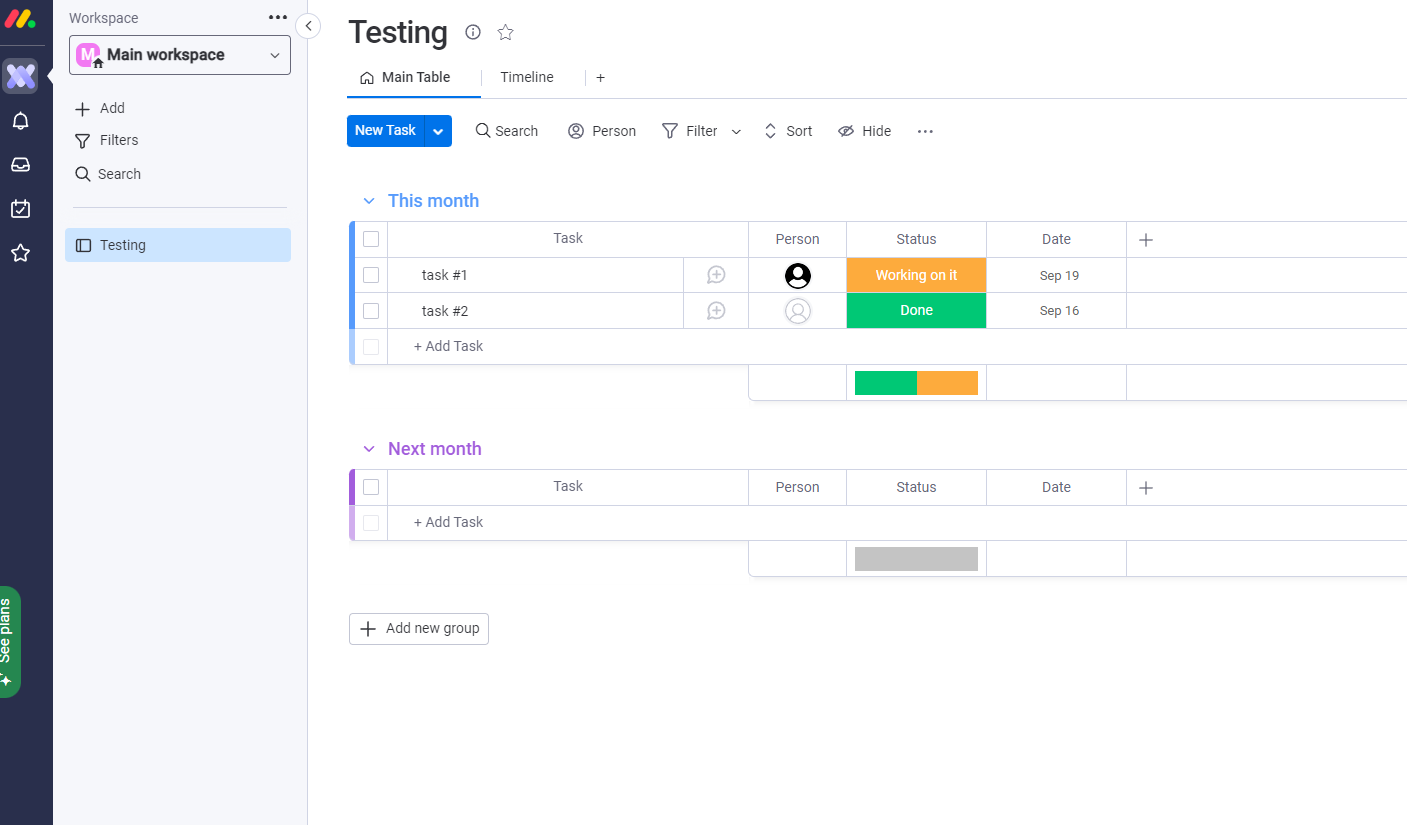
\includegraphics[width=16cm]{../content/images/monday.com/MondayBoard.png}
        \caption{TRELLO board}
    \end{center}
\end{figure}
%------------------------------------------------------- 

In der Standartkonfiguration werden Tasks aufgelistet und nicht als Kanbanboard dargestellt.
Wird ein neuer Workspace erstellt, so klickt man sich erst durch eine Reihe fragen, deren Resultate anschliessend das Layout und die Funktionen
des Workspaces vordefinieren.\\
Die Ansicht des Workspaces ist nach belieben konfigurierbar, so können  Tasks nach Monaten gruppiert werden oder aber auch zB. nach Sprints oder Thema.
Monday.com setzt ebenfalls auf das Freemium Geschäftsmodell, für ein Abo wird jedoch nicht so penetrant geworben wie bei anderen Anbietern.\\
\space
%------------------------------------------------------- 
%TRELLO CARD SCREENSHOT WRAPPER
\begin{wrapfigure}{l}{0.4\textwidth}
    \begin{center}
        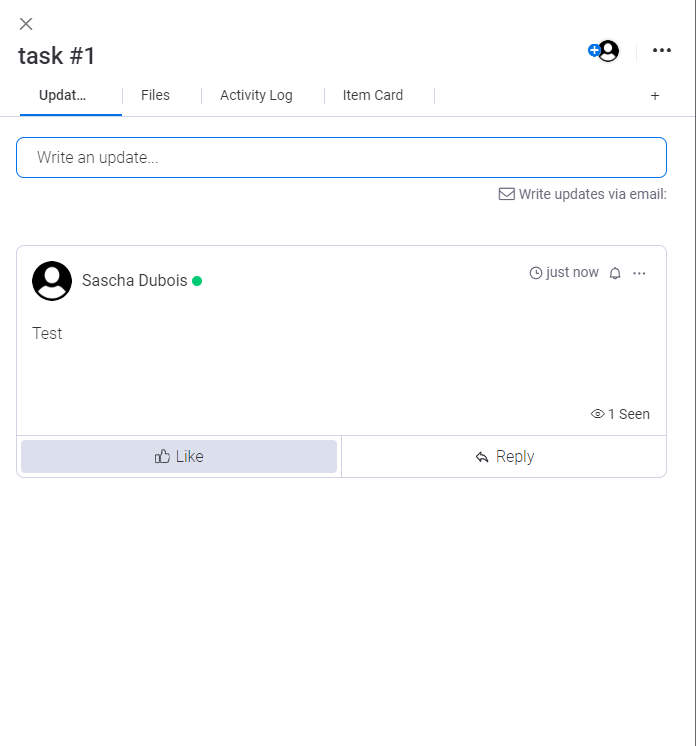
\includegraphics[width=5cm]{../content/images/monday.com/MondayTask.png}
        \caption{Monday.com Task}
    \end{center}
\end{wrapfigure}
%------------------------------------------------------- 

Monday.com können Tasks erstellt werden, im gegensatz zu anderen Anbietern sind diese Tasks
sehr minimalistisch gehalten und enthalten lediglich einen Titel und eine Beschreibung.\\
Den Tasks können jedoch weitere Views angefügt werden, in deren weiter felder und Funktionen zu verfügung stehen.
Vom Prinzip her gleicht es zwar den PowerUps von trello, dort finde ich jedoch die Anbindung um einiges
intuitiver und effizienter.\\

%------------------------------------------------------- 
%TRELLO POWERUPS SCREENSHOT WRAPPER
\begin{figure}[H]
    \begin{center}
        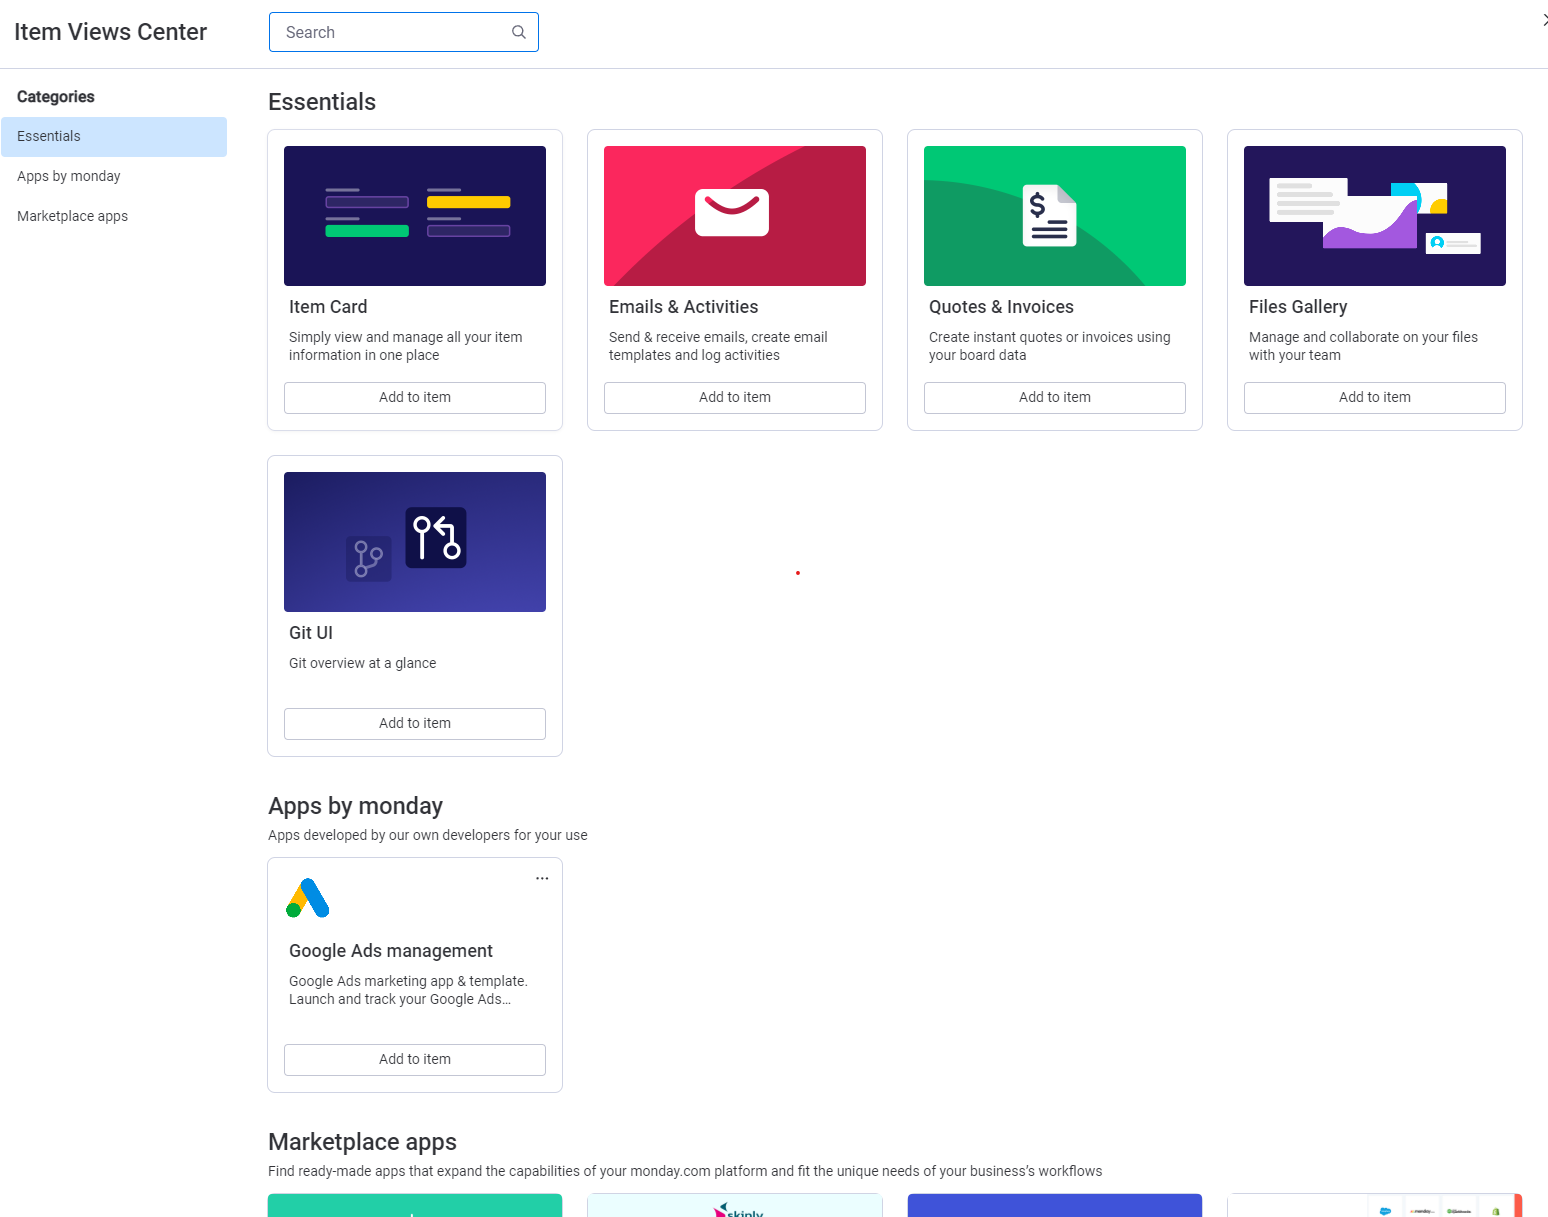
\includegraphics[width=8cm]{../content/images/monday.com/MondayItemViewsCenter.png}
        \caption{TRELLO PowerUps}
    \end{center}
\end{figure}
%------------------------------------------------------- 

Views können im Item-View-Center durchstöbert und hinzugefügt werfden. 
Die hinzugefügten Views erscheinen dann in einem separaten Tab im Task. In den Views ist es ausserdem möglich Widgets einzufügen
und das generelle Layout zu konfigurieren.\\
Im Item-View-Center findet man native Monday.com Views aber auch ausreichend andere Views von drittanbietern.

%------------------------------------------------------- 
%TRELLO DETAILS TABLE
\begin{table}[H]
    \centering
    \settowidth\tymin{executeIncomingCommand()}
    \setlength\extrarowheight{2pt}
    \begin{tabulary}{1.0\textwidth}{|L|L|}
      \hline
      \textbf{Besitzer} &
      monday.com\\
      \hline
      \textbf{Gründung} &
      2012\\
      \hline
      \textbf{Plattform} &
      Web\\
      \hline
      \textbf{Layout} &
      Liste\\
      \hline
      \textbf{Geschäftsmodell} &
      Freemium\\
      \hline
    \end{tabulary}
    \caption{Monday.com Details}
  \end{table}
%------------------------------------------------------- 

%------------------------------------------------------- 
%TRELLO RATING TABLE
\begin{table}[H]
    \centering
    \settowidth\tymin{executeIncomingCommand()}
    \setlength\extrarowheight{2pt}
    \begin{tabulary}{1.0\textwidth}{|L|L|L|}
      \hline
      \textbf{Bewertungspunkt} &
      \textbf{Bewertung} &
      \textbf{Begründung} \\
      \hline
      \textbf{Benutzerfreundlichkeit} &
      ***&
      --\\
      \hline
      \textbf{Darstellung} &
      ****&
     Listenansichten werden schnell unübersichtlich\\
      \hline
      \textbf{Usability} &
      *****&
      Da monday.com eine Webapplikation ist, ist sie auf allen webfähigen Geräten zugänglich + gut optimiert für Mobilgeräte\\
      \hline
      \textbf{Funktionalität} &
      ****&
      Durch Views können Funktionalitäten hinzugefügt werden jedoch ist die auswahl deutlich kleiner als z.B. bei Trello\\
      \hline
      \textbf{Preis} &
      *****&
      Gratis version reicht vollkommen\\
      \hline
    \end{tabulary}
    \caption{TRELLO Bewertung}
  \end{table}
%------------------------------------------------------- 
\space
\textbf{Punkte zur berücksichtigung in eigenem Projekt:}
\begin{itemize}
    \item Lieber keine Listenansicht verwenden
\end{itemize}

  
  